\def\mySecNum{12.1}
\mySection{\mySecNum~Introduction to the Black-Scholes formula}
%-------------- start slide -------------------------------%{{{ 1 Limit of Binomial Tree.
\begin{frame}[fragile,t]
\begin{center}

	The \textcolor{magenta}{Black-Scholes formula} is a limiting case of the binomial formula
	(infinitely many periods) for the price of a European option.

	\vfill
	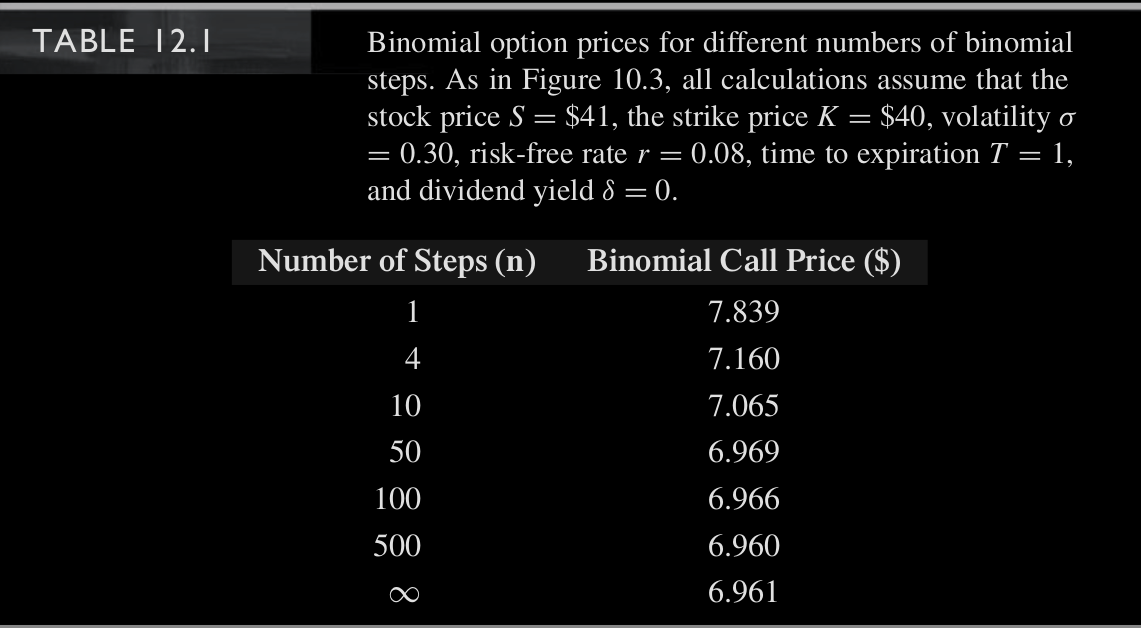
\includegraphics[scale=0.25]{figs/Table-12-1.png}

	\bigskip

	\textcolor{gray}{Check Python code Figure12-1.py}
\end{center}
\end{frame}
%-------------- end slide -------------------------------%}}}
%-------------- start slide -------------------------------%{{{ 1 Formula
\begin{frame}[fragile,t]
	\begin{itemize}
		\item Consider an European call (or put) option written on a stock
		\item Assume that the stock pays dividend at the continuous rate $\delta$
	\end{itemize}
	\pause
	\vfill
	\mySeparateLine

	\begin{minipage}{0.48\textwidth}
	\begin{center}
		Call options
		\begin{gather*}
			C(S,K,\sigma,r,T,\delta) \\ || \\
			S e^{-\delta T}N(d_1)-K e^{-rT}N(d_2)
		\end{gather*}
	\end{center}
	\end{minipage}
	\begin{minipage}{0.48\textwidth}
	\begin{center}
		Put options
		\begin{gather*}
			P(S,K,\sigma,r,T,\delta) \\ || \\
			K e^{-rT}N(-d_2) - S e^{-\delta T}N(-d_1)
		\end{gather*}
	\end{center}
	\end{minipage}
	\bigskip
	\bigskip

	\begin{equation*}
		d_1=\frac{\ln(S/K)+(r-\delta\textcolor{magenta}{+}\frac{1}{2}\sigma^2)T}{\sigma \sqrt{T}} \quad \text{and} \quad
		d_2=\frac{\ln(S/K)+(r-\delta\textcolor{cyan}{-}\frac{1}{2}\sigma^2)T}{\sigma \sqrt{T}}
	\end{equation*}

	\mySeparateLine

	\begin{gather*}
		\text{Put-call Parity}\\
		P = C + Ke^{-rT} - S e^{-\delta T} \\[1em]
		d_1-d_2=\sigma \sqrt{T}
	\end{gather*}
	\bigskip
\end{frame}
%-------------- end slide -------------------------------%}}}
%-------------- start slide -------------------------------%{{{ 1 N(z)
\begin{frame}[fragile,t]
	\begin{align*}
		N(z) = \frac{1}{\sqrt{2\pi}} \int_{-\infty}^z e^{-\frac{x^2}{2}} dx
	\end{align*}
\end{frame}
%-------------- end slide -------------------------------%}}}
%-------------- start slide -------------------------------%{{{ 1 Verification
\begin{frame}[fragile,t]
\begin{myexample}
Verify that the Black-Scholes formula for call and put
\begin{align*}
	C:= C(S,K,\sigma,r,T,\delta) & = S e^{-\delta T}N(d_1)-K e^{-rT}N(d_2) \\
	P:= P(S,K,\sigma,r,T,\delta)  & = K e^{-rT}N(-d_2) - S e^{-\delta T}N(-d_1)
\end{align*}
with
\begin{align*}
	d_i=\frac{\ln(S/K)+(r-\delta\textcolor{magenta}{-(-1)^i}\frac{1}{2}\sigma^2)T}{\sigma \sqrt{T}}, \quad i=1,2
\end{align*}
satisfies the call-put parity: $C - P = S e^{-\delta T} - K e^{-r T}$.
\end{myexample}
\begin{mysol}
	\phantom{a}\\
	\vfill\myEnd
\end{mysol}
\end{frame}
%-------------- end slide -------------------------------%}}}
%-------------- start slide -------------------------------%{{{ 1
\begin{frame}[fragile,t]
	\begin{myexample}
		Plot the functions
		\begin{align*}
			S \to C(S,K,\sigma,r,T-t,\delta) & = S e^{-\delta (T-t)}N(d_1)-K e^{-r(T-t)}N(d_2) \\
			S \to P(S,K,\sigma,r,T-t,\delta)   & = K e^{-r(T-t)}N(-d_2) - S e^{-\delta (T-t)}N(-d_1)
		\end{align*}
		where
		\begin{equation*}
			d_1=\frac{\ln(S/K)+(r-\delta\textcolor{magenta}{+}\frac{1}{2}\sigma^2)(T-t)}{\sigma \sqrt{T-t}} \quad \text{and} \quad
			d_2=\frac{\ln(S/K)+(r-\delta\textcolor{cyan}{-}\frac{1}{2}\sigma^2)(T-t)}{\sigma \sqrt{T-t}}
		\end{equation*}
		with $\sigma, r, \delta, K$ fixed for various values of $T-t=2, 1.5, 1, 0.5, 0$.
	\end{myexample}
	\bigskip
	\begin{mysol}
		Try code \\
		\begin{center}
			\textcolor{gray}{CallPut\_vs\_T-t.nb}
		\end{center}
		\myEnd
	\end{mysol}
\end{frame}
%-------------- end slide -------------------------------%}}}
%-------------- start slide -------------------------------%{{{ 1 Example
\begin{frame}[fragile,t]
\begin{myexample}
	Let $S=\$41$,	$K=\$40$,  $\sigma=0.3$, $r=8\%$,  $T=0.25$ (3 months), and $\delta=0$. Compute the
	Black-Scholes call and put prices. Compare what you obtained with the results obtained from the
	binomial tree.
\end{myexample}
\vfill
\begin{center}
	Check code \\
	\textcolor{gray}{Example12-1.py}
\end{center}
\end{frame}
%-------------- end slide -------------------------------%}}}
%-------------- start slide -------------------------------%{{{ Code -- Removed.
% \begin{frame}[fragile,t]
% 	\begin{center}
% 		\textcolor{gray}{Try code:\\ Example12-1.py}
% 	\end{center}
% 	\bigskip
% 	\begin{lstlisting}
% 	import numpy as np
% 	from scipy.stats import norm
%
% 	# Input the parameters{{{
% 	S = 41
% 	K = 40
% 	sigma = 0.30
% 	r = 0.08
% 	T = 0.25
% 	delta = 0.00
% 	# }}}
%
% 	d1 = (np.log(S/K)+(r-delta+pow(sigma, 2)/2)*T)/(sigma * np.sqrt(T))
% 	d2 = d1 - sigma * np.sqrt(T)
% 	BS_Call = S * np.exp(-delta * T) * norm.cdf(d1) - K * np.exp(-r * T) * norm.cdf(d2)
% 	BS_Put= K * np.exp(- r * T) * norm.cdf(-d2) - S * np.exp(-delta * T) * norm.cdf(-d1)
% 	print("Option prices for call and put computed by Black-Schole model for Examples 12.1 and 12.2 are equal to")
% 	print("{:4.4f} and {:4.4f}, respectively.".format(BS_Call, BS_Put))
% 	\end{lstlisting}
% 	\vfill
% 	\begin{lstlisting}
% 	3.3991 and 1.6070, respectively.
% 	\end{lstlisting}
% \end{frame}
%-------------- end slide -------------------------------%}}}
%-------------- start slide -------------------------------%{{{ 1 Assumptions
\begin{frame}[fragile,t]
	\frametitle{When is the Black-Scholes formula valid?}

	Assumptions about \textcolor{magenta}{stock return distribution}
\bigskip
\begin{itemize}
	\item Continuously compounded returns on the stock are normally distributed and independent over time (no “jumps”)
	\item The volatility of continuously compounded returns is known and constant
	\item Future dividends are known, either as dollar amount or as a fixed dividend yield
\end{itemize}

\pause
\bigskip
\mySeparateLine
\bigskip

Assumptions about the \textcolor{cyan}{economic environment}
\bigskip

\begin{itemize}
	\item The risk-free rate is known and constant
	\item There are no transaction costs or taxes
	\item It is possible to short-sell costlessly and to borrow at the risk-free rate
\end{itemize}
\end{frame}
%-------------- end slide -------------------------------%}}}
